\documentclass[tikz, border = 10pt]{standalone}


\usepackage{newpxtext,newpxmath}   % /upbeta
%\usepackage{fouriernc}            % /otherbeta
\usepackage{amsmath}
\renewcommand{\familydefault}{\sfdefault}
\usepackage{mathastext}

\usetikzlibrary{positioning, quotes, calc, math, arrows.meta, bending, shapes, backgrounds}

\tikzset{
every edge quotes/.style = {fill = white},
every node/.style = {scale = 1.1},
manifest/.style = {rectangle, draw, thin, inner sep = 3pt, minimum width = 1cm,
   minimum height = .85cm, align = center},
latent/.style = {ellipse, draw, thin, inner sep = 3pt, minimum width = 1cm,
   minimum height = .85cm},
residual1/.style = {circle, draw, thin, minimum size = 5mm, inner sep = 1pt},
residual2/.style = {rectangle, minimum width = 0.5pt, minimum height = 1.5mm,
   inner sep = 0pt, outer sep = 0mm},
regression/.style = {-{Stealth[length = 1.5mm]}, thin, shorten > = 1pt, 
   inner sep = 1.5pt, outer sep = 0mm},
covariance/.style={{Stealth[length = 1.5mm]}-{Stealth[length = 1.5mm]}, thin,
   shorten > = 1pt, shorten < = 1pt, inner sep = 1.5pt},
variance/.style={{Stealth[length = 1mm]}-{Stealth[length = 1mm]}, thin,
   shorten > = 1pt, shorten < = 1pt, inner sep = 1pt},
interaction/.style = {-{Stealth[sep = 1pt, length = 1.5mm] . Circle[length = 4pt]},
   thin, shorten > = -2pt},
constant/.style = {draw, thin, inner sep = 1pt, regular polygon,
   regular polygon sides = 3, minimum size = 5mm},
group/.style = {rectangle, inner sep = 2pt, minimum width = 15mm, minimum height = 5mm, 
   align = center}
}

\begin{document}
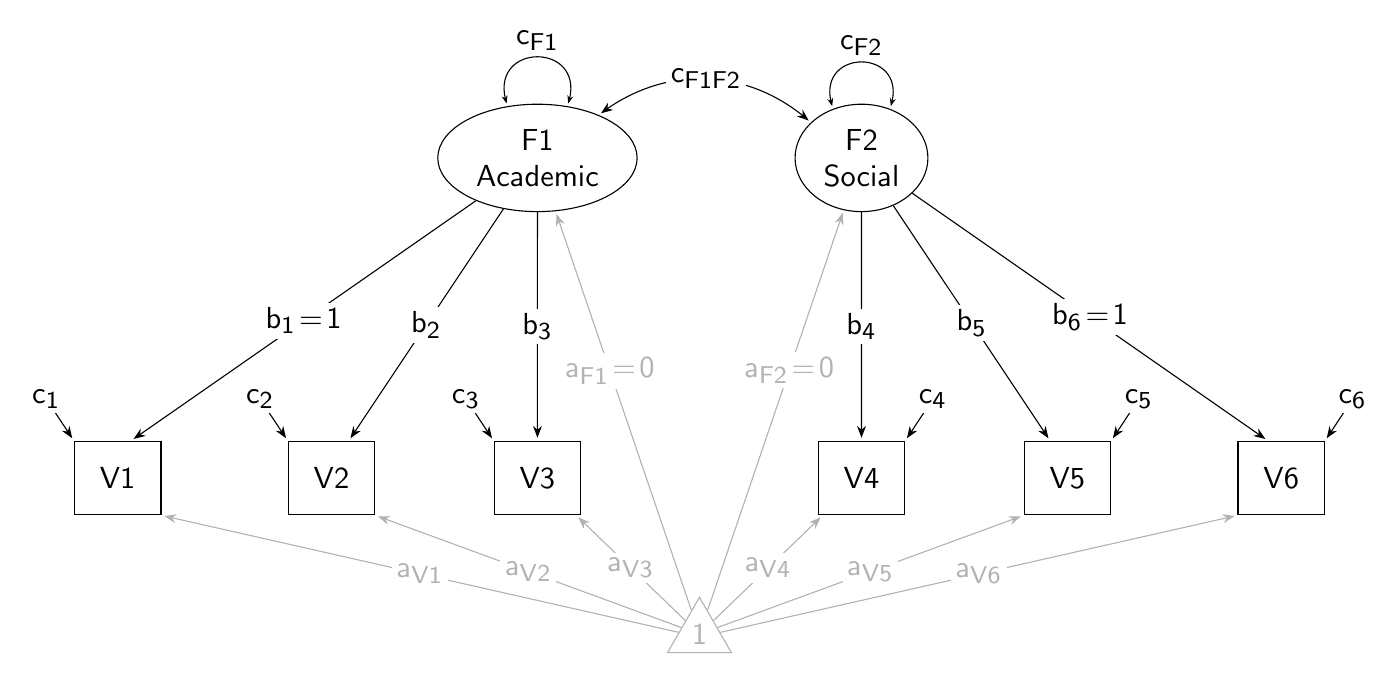
\begin{tikzpicture}

%% Academic manifests
\node [manifest] (V1) {V1};
\node [manifest] (V2) [right = 1.6cm of V1] {V2};
\node [manifest] (V3) [right = 1.5cm of V2] {V3};

%% Social manifests
\node [manifest] (V4) [right = 3cm of V3] {V4};
\node [manifest] (V5) [right = 1.5cm of V4] {V5};
\node [manifest] (V6) [right = 1.6cm of V5] {V6};

%% Academic and Social latents
\node [latent, align=center] (F1) [above = 2.9cm of V3] {F1\\Academic};
\node [latent, align=center] (F2) [above = 2.9cm of V4] {F2\\Social};

%% Loadings
\path [regression] (F1) edge ["b$_1\!=\!1$"] (V1.70);
\path [regression] (F1) edge ["b$_2$"] (V2.65);
\path [regression] (F1) edge ["b$_3$"] (V3.90);

\path [regression] (F2) edge ["b$_4$"] (V4.90);
\path [regression] (F2) edge ["b$_5$"] (V5.115);
\path [regression] (F2) edge ["b$_6\!=\!1$"] (V6.110);

%% Latent variances ans covariance
\path [covariance] (F1.35) edge ["c$_{F1F2}$", bend left = 40] (F2.145);
\path [variance] (F1.120) edge ["c$_{F1}$", above, outer sep = 1pt, bend left = 110, looseness = 3] (F1.60);
\path [variance] (F2.120) edge ["c$_{F2}$", above, outer sep = 1pt, bend left = 110, looseness = 3] (F2.60);

%% Residuals
\node [residual2] (e1) [above left = .65cm of V1, xshift = 1mm] {};
\path [regression] (e1) edge ["c$_1$", pos = 0] (V1.north west);

\node [residual2] (e2) [above left = .65cm of V2, xshift = 1mm] {};
\path [regression] (e2) edge ["c$_2$", pos = 0] (V2.north west);

\node [residual2] (e3) [above left = .65cm of V3, xshift = 1mm] {};
\path [regression] (e3) edge ["c$_3$", pos = 0] (V3.north west);

\node [residual2] (e4) [above right = .65cm of V4, xshift = -1mm] {};
\path [regression] (e4) edge ["c$_4$", pos = 0] (V4.north east);

\node [residual2] (e5) [above right = .65cm of V5, xshift = -1mm] {};
\path [regression] (e5) edge ["c$_5$", pos = 0] (V5.north east);

\node [residual2] (e6) [above right = .65cm of V6, xshift = -1mm] {};
\path [regression] (e6) edge ["c$_6$", pos = 0] (V6.north east);

%% Latent means
\node [constant, black!30] (M) [below = 1.5cm of $(V3)!0.5!(V4)$] {1};
\path [regression, black!30] (M) edge ["a$_{F1}\!=\!0$", pos = .6] (F1);
\path [regression, black!30] (M) edge ["a$_{F2}\!=\!0$", pos = .6] (F2);

%% Intercepts
\path [regression, black!30] (M.175) edge ["a$_{V1}$"] (V1.south east);
\path [regression, black!30] (M) edge ["a$_{V2}$"] (V2.south east);
\path [regression, black!30] (M) edge ["a$_{V3}$"] (V3);

\path [regression, black!30] (M) edge ["a$_{V4}$"] (V4);
\path [regression, black!30] (M) edge ["a$_{V5}$"] (V5.south west);
\path [regression, black!30] (M.5) edge ["a$_{V6}$"] (V6.south west);

\end{tikzpicture}
\end{document}

